\documentclass{beamer}
\usetheme{Darmstadt}
\usecolortheme{beaver}
\usepackage{listings}
\usepackage[utf8]{inputenc}
\usepackage[french]{babel}
\usepackage{xcolor,colortbl}



\begin{document}

\author{Rémy \textsc{El Sibaïe Besognet}}
\title{Bibliothèque OCaml pour la combinatoire}
\date{\today}

\begin{frame}
  \titlepage
\end{frame}

%%% 1 EMC
\begin{frame}{Exact Matrix Covering}

Problème EMC ou couverture exacte de matrice :


 \begin{columns}

    \column{0.5\textwidth}
				\begin{itemize}
				\item Un sous-ensemble de lignes avec un et un seul 1 par colonne
				\item Problème difficile
				\end{itemize}

    \column{0.5\textwidth}
  \begin{displaymath}
   \left(\begin{array}{ c c c c c }
   1 & 0 & 1 & 1 \\
   0 & 1 & 1 & 0 \\
   1 & 1 & 0 & 1 \\
   1 & 0 & 0 & 1 \\
   0 & 1 & 0 & 0
  \end{array}\right)
  \end{displaymath}

  \end{columns}
\end{frame}


\begin{frame}{EMC : exemple}

\begin{displaymath}
   \left(\begin{array}{ c c c c c }
   1 & 0 & 1 & 1 \\
   0 & 1 & 1 & 0 \\
   1 & 1 & 0 & 1 \\
   1 & 0 & 0 & 1 \\
   0 & 1 & 0 & 0
  \end{array}\right)
  \end{displaymath}

\begin{center}
$ \{3, 4\} $ n'est pas une solution\\
$ \{0, 4\}, \{1, 3\} $ sont des solutions
\end{center}
\end{frame}

\begin{frame}{Application : Pavage avec des dominos}

\begin{center}
  \begin{tabular}{|c|c|c|c|}
		\hline
   	\cellcolor{red} & \cellcolor{red} &  &  \\
		\hline
    	&  &  &  \\
		\hline
   	 &  &  &  \\
		\hline
   & &  &  \\
		\hline
\end{tabular}
\end{center}


Poser un domino sur les cases 0-1 :
\[
  \begin{array}{ c c c c c c c c c c c c c c c c }
	1 & 1 & 0 & 0 & 0 & 0 & 0 & 0 & 0 & 0 & 0 & 0 & 0 & 0 & 0 & 0 
  \end{array}
\]
\end{frame}



\begin{frame}{Application : Sudoku}

\begin{figure}[h]
\scalebox{0.7}{
\centering

$\begin{array}{|c|c|c||c|c|c||c|c|c|}
\hline
5 & 3 &   &   & 7 &   &  &   &    \\
\hline
6 &   &   & 1 & 9 & 5 &  &   &    \\
\hline
  & 9 & 8 &   &   &   &  & 6 &    \\
\hline
\hline
8 &   &   &   & 6 &   &   &   & 3 \\
\hline
4 &   &   & 8 &   & 3 &   &   & 1 \\
\hline
7 &   &   &   & 2 &   &   &   & 6 \\
\hline
\hline
  & 6 &   &   &   &   & 2 & 8 &   \\
\hline
  &   &   & 4 & 1 & 9 &   &   & 9 \\
\hline
  &   &   &   & 8 &   &   & 7 & 5 \\
\hline
\end{array}$
}
\end{figure}

324 colonnes : 
\begin{enumerate}
\item 81 cases dans un Sudoku
\item $ 9~\textrm{lignes} \times 9~\textrm{valeurs}$ 
\item $ 9~\textrm{colonnes} \times 9~\textrm{valeurs}$ 
\item $ 9~\textrm{cellules} \times 9~\textrm{valeurs}$
\end{enumerate}



\end{frame}





\begin{frame}{Application : N-Reines}
\begin{figure}[h]
\begin{center}
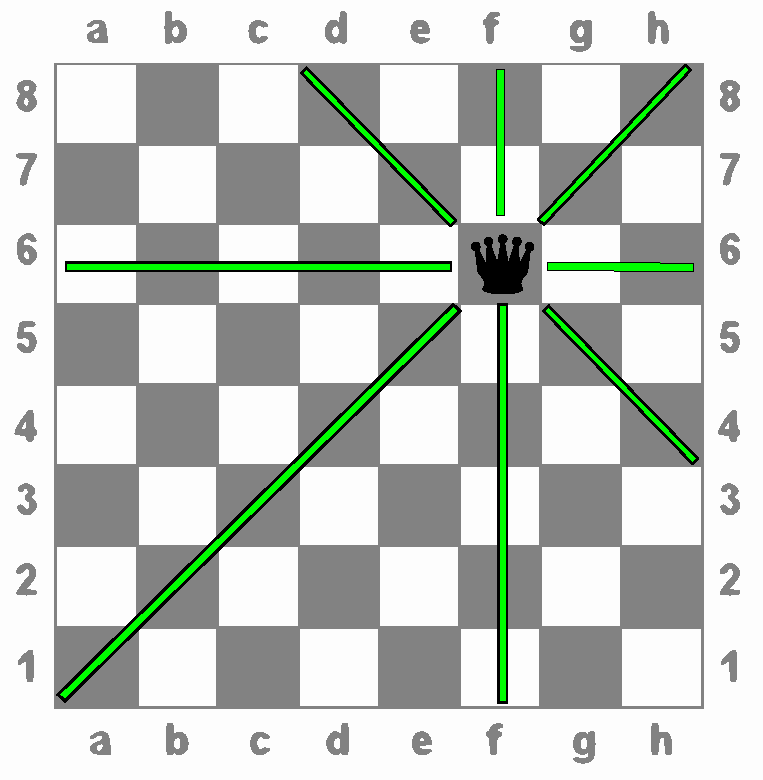
\includegraphics[height=0.4\textheight]{../imports/8queens.pdf}
\end{center}
\end{figure}

46 colonnes : 
\begin{itemize}
\item 8 lignes
\item 8 colonnes
\item 15 diagonales gauche-droite
\item 15 diagonales droite-gauche
\end{itemize}


\end{frame}

 \begin{frame}{Deux techniques pour résoudre EMC}

\begin{enumerate}
\item Dancing Links
\item ZDD 
\end{enumerate}




\end{frame}
%%% 2 DLX
\begin{frame}{Dancing Links de Knuth}

The Dancing Links ou DLX\\
Une utilisation astucieuse des listes doublements chaînées : 
\begin{figure}[h]
\begin{center}
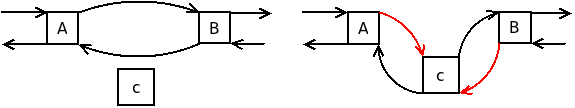
\includegraphics[scale=0.5]{../imports/add_elmt_dll.png}
\end{center}
\end{figure}
\end{frame}

\begin{frame}{Principe de base de DLX}
Suppression puis ré-ajout
\begin{figure}[h]
\begin{center}
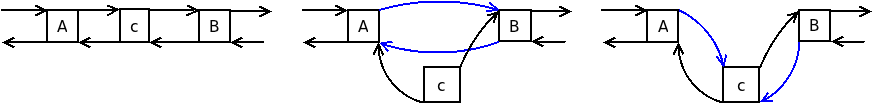
\includegraphics[scale=0.3]{../imports/delete.png}
\end{center}
\end{figure}
\end{frame}

\begin{frame}{Une structure exotique}

La matrice doublement chaînée

 \begin{columns}
    \column{0.5\textwidth}
\begin{center}$
\left(\begin{array}{ c c c c c }
   1 & 1 \\
   1 & 0 
  \end{array}\right)$
\end{center}

    \column{0.5\textwidth}
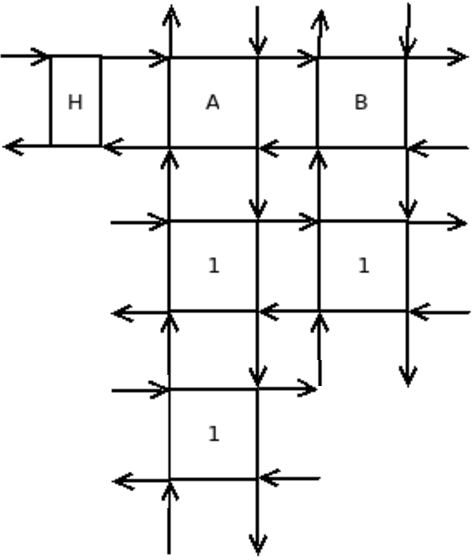
\includegraphics[scale=0.4]{../imports/dlx_matrice.pdf}
 \end{columns}

%Présence d'en-têtes, circulaire, contient uniquement les 1 de EMC.
\end{frame}


%%% 3 ZDD
\begin{frame}{Zero-Suppressed Binary Decision Diagram (ZDD)}
Une variante de BDD\\

\begin{center}
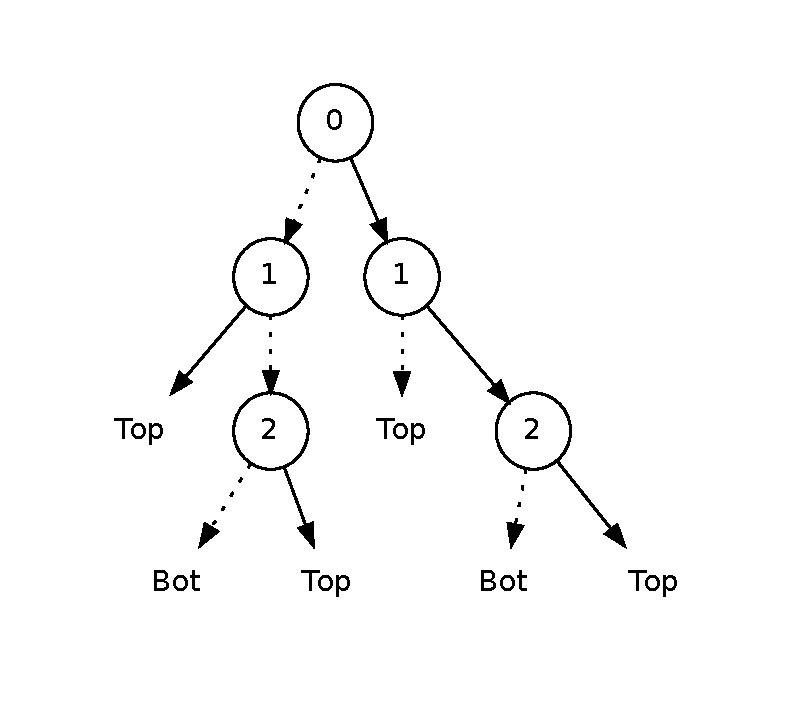
\includegraphics[scale=0.3]{../imports/zdd_ex.pdf}
\end{center}
\begin{itemize}
\item Pas de $\bot$ à droite
\item Valeur des n\oe uds croissante en descendant
\end{itemize} 
\end{frame}


\begin{frame}{Un ensemble d'ensembles}
Sur l'ensemble $E = \{0, 1,..,n - 1\}$
\begin{figure}[htp]
\begin{center}
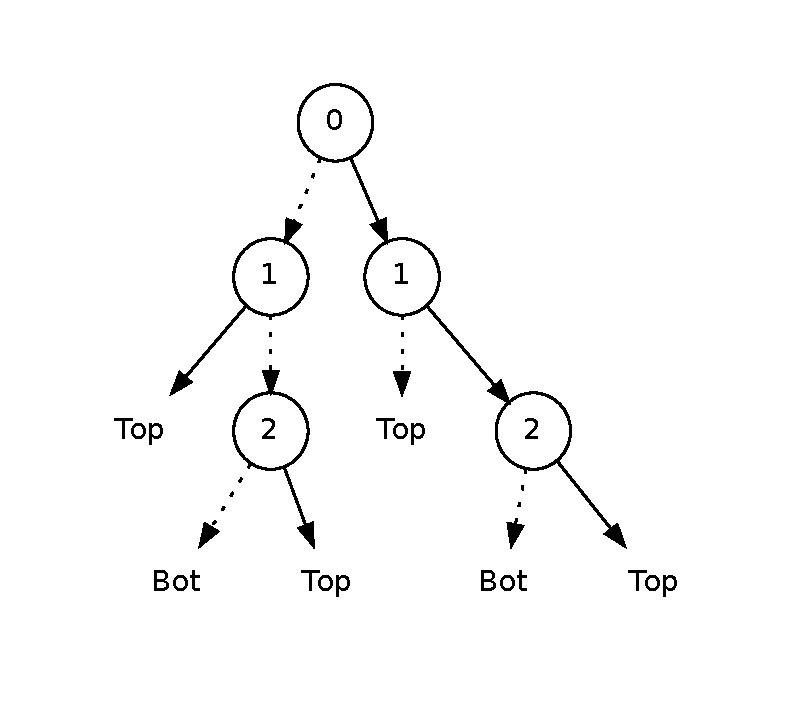
\includegraphics[scale=0.3]{../imports/zdd_ex.pdf}
\end{center}
\end{figure}
correspond à \{\{0, 1, 2\}, \{0\}, \{1\}, \{2\}\}
\end{frame}


\begin{frame}{ZDD : Optimisations}
Comme pour les BBD 
\begin{enumerate}
\item partage des sous-arbres communs (\emph{hash consing})
\begin{center}
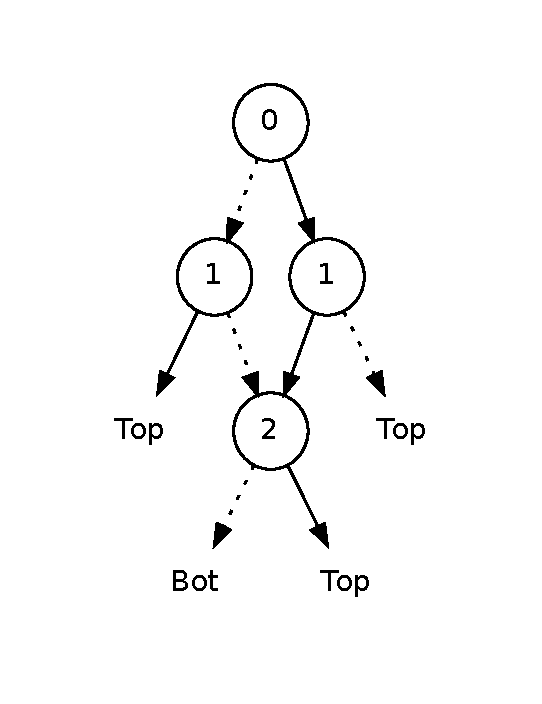
\includegraphics[scale=0.4]{../imports/zdd_construct.pdf}
\end{center}
\item \emph{mémoïzation} des opérations sur les ZDD
\end{enumerate}


\end{frame}

\begin{frame}{EMC vers ZDD}
  \begin{columns}
    \column{0.5\textwidth}

  \begin{displaymath}
   \left(\begin{array}{ c c c c c }
   1 & 0 & 1 &\cellcolor{red} 1 \\
   0 & 1 & 1 &\cellcolor{red} 0 \\
   1 & 1 & 0 &\cellcolor{red} 1 \\
   1 & 0 & 0 &\cellcolor{red} 1 \\
   0 & 1 & 0 &\cellcolor{red} 0
  \end{array}\right)
  \end{displaymath}

    \column{0.5\textwidth}
    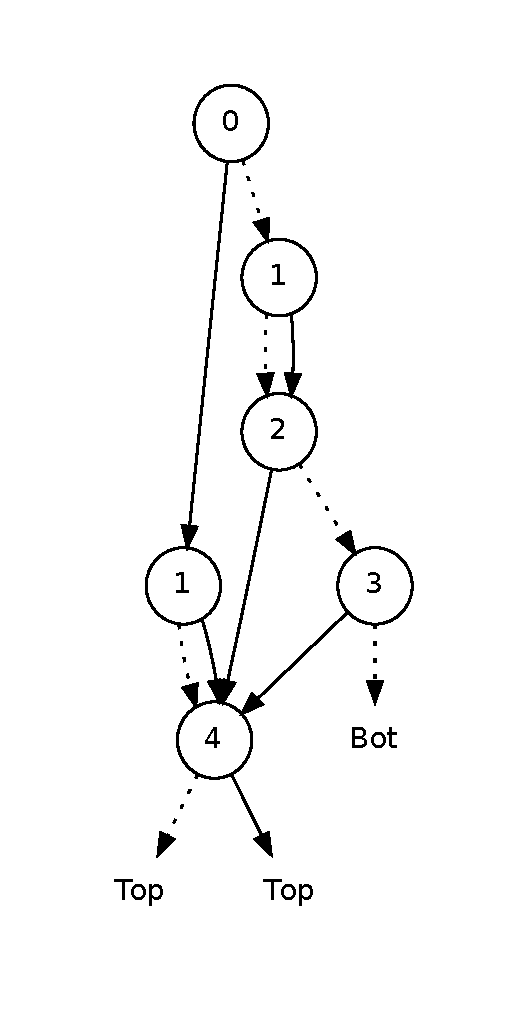
\includegraphics[height=0.9\textheight]{../imports/column.pdf}
  \end{columns}
\end{frame}

\begin{frame}{Réduction vers EMC : après intersection}
  \begin{columns}
    \column{0.3\textwidth}

  \begin{displaymath}
   \left(\begin{array}{ c c c c c }
   1 & 0 & 1 & 1 \\
   0 & 1 & 1 & 0 \\
   1 & 1 & 0 & 1 \\
   1 & 0 & 0 & 1 \\
   0 & 1 & 0 & 0
  \end{array}\right)
  \end{displaymath}

    \column{0.7\textwidth}
    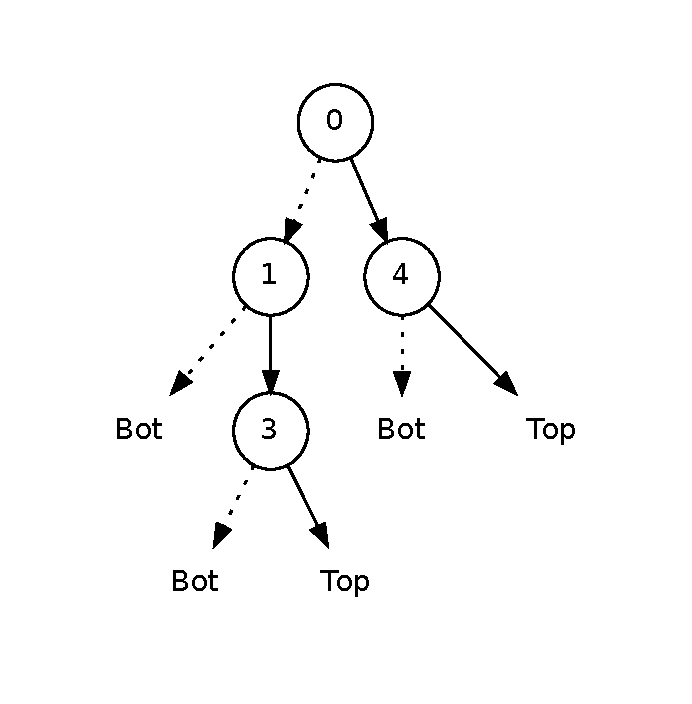
\includegraphics[height=0.8\textheight]{../imports/inter.pdf}
  \end{columns}
\end{frame}

\begin{frame}{}
\begin{center}
    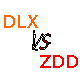
\includegraphics[height=0.5\textheight]{../imports/vs.pdf}
\end{center}
\begin{itemize}
\item DLX : rapide mais trouver les solutions une à une.
\item ZDD : avantage en temps mais peut faire exploser la mémoire \\
\end{itemize}
~\\
Conclusion : dépend du problème et/ou de la question.
\end{frame}



%%% 4 bibliothèque OCaml
\begin{frame}{ReMl : une bibliothèque OCaml}
\begin{itemize}
\item Outils pour résoudre EMC
\item Outils pour encoder dans EMC
\item Un mini langage pour le pavage
\end{itemize}
\end{frame}


\begin{frame}{ReMl : Architecture des modules}
\begin{figure}[htp]
\begin{center}
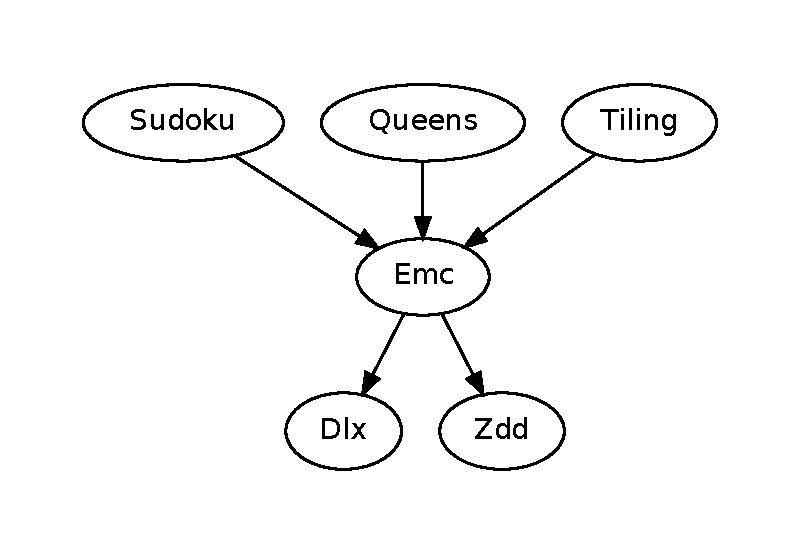
\includegraphics[scale=0.5]{../imports/archi_slide.pdf}
\end{center}
\end{figure}
\end{frame}

\begin{frame}[fragile]{ReMl : Un mini langage pour le pavage}

Problème sous forme de patrons : 
\begin{columns}
    \column{0.3\textwidth}
\begin{lstlisting}
pattern b = {
**
.*
**
}
\end{lstlisting}
    \column{0.1\textwidth}
		$\rightarrow$
    \column{0.3\textwidth}
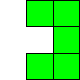
\includegraphics[scale=1]{../imports/patron.pdf}
\end{columns}
\end{frame}

\begin{frame}{ReMl : définir un problème}

\lstinputlisting[language=Caml]{../imports/non-regression.rem}

\#options :  
\emph{$\sim$sym}, \emph{$\sim$one} ou \emph{$\sim$maybe}
 
 \end{frame}


\begin{frame}{ReMl : les isométries}

Les 8 isométries du carré : \\
~\\

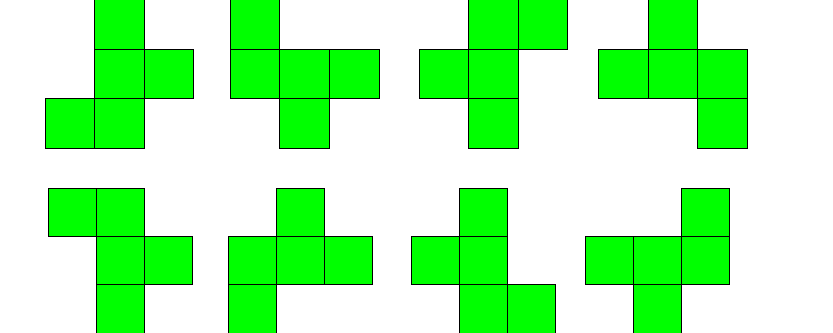
\includegraphics[scale=0.5]{../imports/transformations.pdf}
\end{frame}




\begin{frame}{Conclusion}

Résultats :  
\begin{itemize}
\item Des algorithmes qui fonctionnent (résultats cohérents)
\item Une bibliothèque facile d'utilisation
\end{itemize}

Pour aller plus loin : 
\begin{itemize}
\item Optimisations des calculs en fonction des symétries du problème
\item Ajout de fonctionnalités dans le langage
\item Documentation
\end{itemize}



\end{frame}

\end{document}
